%%%%%%%%%%%%%%%%%%%%%%%%%%%%%%%%%%%%%%%%%
% Structured General Purpose Assignment
% LaTeX Template
%
% This template has been downloaded from:
% http://www.latextemplates.com
%
% Original author:
% Ted Pavlic (http://www.tedpavlic.com)
%
% Note:
% The \lipsum[#] commands throughout this template generate dummy text
% to fill the template out. These commands should all be removed when 
% writing assignment content.
%
%%%%%%%%%%%%%%%%%%%%%%%%%%%%%%%%%%%%%%%%%

%----------------------------------------------------------------------------------------
%	PACKAGES AND OTHER DOCUMENT CONFIGURATIONS
%----------------------------------------------------------------------------------------

\documentclass{article}

\usepackage{fancyhdr} % Required for custom headers
\usepackage{lastpage} % Required to determine the last page for the footer
\usepackage{extramarks} % Required for headers and footers
\usepackage{graphicx} % Required to insert images
\usepackage{caption}
\usepackage{float}
\usepackage{hyperref}
\usepackage{subcaption}


% Margins
\topmargin=-0.45in
\evensidemargin=0in
\oddsidemargin=0in
\textwidth=6.5in
\textheight=9.0in
\headsep=0.25in 


\linespread{1.1} % Line spacing

% Set up the header and footer
\pagestyle{fancy}
\lhead{\hmwkAuthorName} % Top left header
\chead{\hmwkClass\ \hmwkTitle} % Top center header
\rhead{\firstxmark} % Top right header
\lfoot{\lastxmark} % Bottom left footer
\cfoot{} % Bottom center footer
\rfoot{Page\ \thepage\ of\ \pageref{LastPage}} % Bottom right footer
\renewcommand\headrulewidth{0.4pt} % Size of the header rule
\renewcommand\footrulewidth{0.4pt} % Size of the footer rule

\setlength\parindent{0pt} % Removes all indentation from paragraphs

%----------------------------------------------------------------------------------------
%	DOCUMENT STRUCTURE COMMANDS
%	Skip this unless you know what you're doing
%----------------------------------------------------------------------------------------

% Header and footer for when a page split occurs within a problem environment
\newcommand{\enterProblemHeader}[1]{
\nobreak\extramarks{#1}{#1 continued on next page\ldots}\nobreak
\nobreak\extramarks{#1 (continued)}{#1 continued on next page\ldots}\nobreak
}

% Header and footer for when a page split occurs between problem environments
\newcommand{\exitProblemHeader}[1]{
\nobreak\extramarks{#1 (continued)}{#1 continued on next page\ldots}\nobreak
\nobreak\extramarks{#1}{}\nobreak
}

\setcounter{secnumdepth}{0} % Removes default section numbers
\newcounter{homeworkProblemCounter} % Creates a counter to keep track of the number of problems

\newcommand{\homeworkProblemName}{}
\newenvironment{homeworkProblem}[1][Problem \arabic{homeworkProblemCounter}]{ % Makes a new environment called homeworkProblem which takes 1 argument (custom name) but the default is "Problem #"
\stepcounter{homeworkProblemCounter} % Increase counter for number of problems
\renewcommand{\homeworkProblemName}{#1} % Assign \homeworkProblemName the name of the problem
\section{\homeworkProblemName} % Make a section in the document with the custom problem count
\enterProblemHeader{\homeworkProblemName} % Header and footer within the environment
}{
\exitProblemHeader{\homeworkProblemName} % Header and footer after the environment
}

\newcommand{\problemAnswer}[1]{ % Defines the problem answer command with the content as the only argument
\noindent\framebox[\columnwidth][c]{\begin{minipage}{0.98\columnwidth}#1\end{minipage}} % Makes the box around the problem answer and puts the content inside
}

\newcommand{\homeworkSectionName}{}
\newenvironment{homeworkSection}[1]{ % New environment for sections within homework problems, takes 1 argument - the name of the section
\renewcommand{\homeworkSectionName}{#1} % Assign \homeworkSectionName to the name of the section from the environment argument
\subsection{\homeworkSectionName} % Make a subsection with the custom name of the subsection
\enterProblemHeader{\homeworkProblemName\ [\homeworkSectionName]} % Header and footer within the environment
}{
\enterProblemHeader{\homeworkProblemName} % Header and footer after the environment
}
   
%----------------------------------------------------------------------------------------
%	NAME AND CLASS SECTION
%----------------------------------------------------------------------------------------

\newcommand{\hmwkTitle}{"Fishing Association Website Prototype"} % Assignment title
\newcommand{\hmwkDueDate}{Tuesday,\ April\ 22,\ 2014} % Due date
\newcommand{\hmwkClass}{CS\ 22310} % Course/class
\newcommand{\hmwkAuthorName}{James Euesden - jee22} % Your name

%----------------------------------------------------------------------------------------
%	TITLE PAGE
%----------------------------------------------------------------------------------------

\title{
\vspace{2in}
\textmd{\textbf{\hmwkClass:\ \hmwkTitle}}\\
\normalsize\vspace{0.1in}\small{Due\ on\ \hmwkDueDate}\\
\vspace{3in}
}

\author{\textbf{\hmwkAuthorName}}
\date{} % Insert date here if you want it to appear below your name

%----------------------------------------------------------------------------------------

\setlength\parindent{24pt}

\begin{document}

\maketitle

%----------------------------------------------------------------------------------------
%	TABLE OF CONTENTS
%----------------------------------------------------------------------------------------

%\setcounter{tocdepth}{1} % Uncomment this line if you don't want subsections listed in the ToC

\newpage
\tableofcontents
\newpage

%----------------------------------------------------------------------------------------
%	INTRODUCTION
%----------------------------------------------------------------------------------------

% To have just one problem per page, simply put a \clearpage after each problem

\section{Introduction}
For this task, I was provided a Requirements Specification\cite{assignment} about a new website for the fictional 'Consolidated Fishing Association'. In this scenario, the association wishes to have a new website designed to boost their profits through pooling batches of caught fish together into auction lots that are hosted on an online auction application and sold to the highest bidder. My task was to use this specification and take the idea through to the prototype stage.

The resulting prototype can be found:

\url{http://users.aber.ac.uk/jee22/cs22310/index.html}

See the 'Prototype' section for gaining access to the website via the login box.


%----------------------------------------------------------------------------------------
%	TASK ANALYSIS
%----------------------------------------------------------------------------------------

\section{Task Analysis}
Beginning with the task analysis in the requirements specification, I took a look at who the users of the application would be, what their needs were and what tasks the application should fulfill in order to meet their expectations.
\subsection{Who is involved?}
From studying the functional requirements of the application, it was clear that there were four main types of users.
\begin{itemize}
\item Fishermen, who catch the batches of fish, bring them to the warehouse, upload data about their batches to the website database and then label the batches accordingly.
\item Warehouse staff members that look at all of the currently available batches on the website and create auction lots out of them, based on the species and weights.
\item Buyers who wish to bid on the auctions and buy the lots of fish.
\item Administrative staff members that have the ability to add new users of different types to the system.
\end{itemize}

To further demonstrate the users and what they require, here is a picture representation:
\begin{figure}[H]
	\centering
	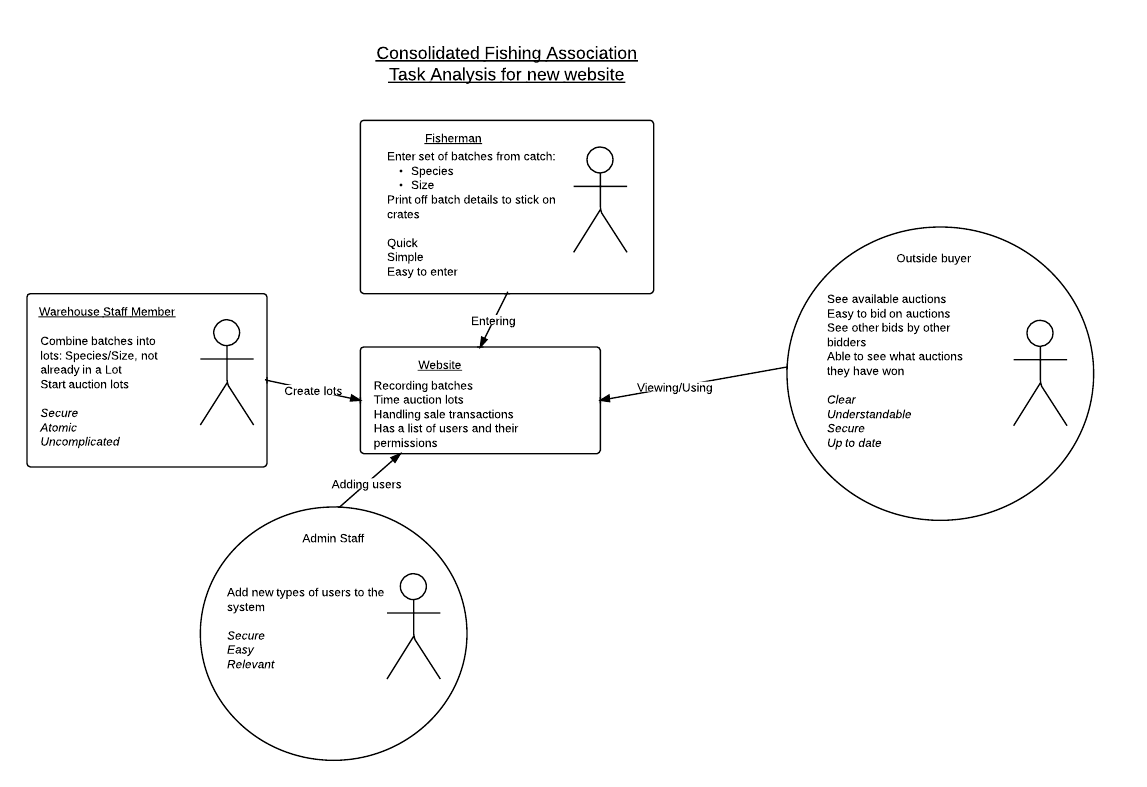
\includegraphics[width=0.8\textwidth]{img/TA-RP1.png}
	\caption{A rich picture to show who the users are and what they require from the system}
\end{figure}
\subsection{Use Case Diagram}
From further  examination of the functional requirements, I found it useful to draft up a Use Case diagram, displaying the basic needs of each individual person who will be using the application, and what might be needed for them to accept this application into their daily routine.

\begin{figure}[H]
	\centering
	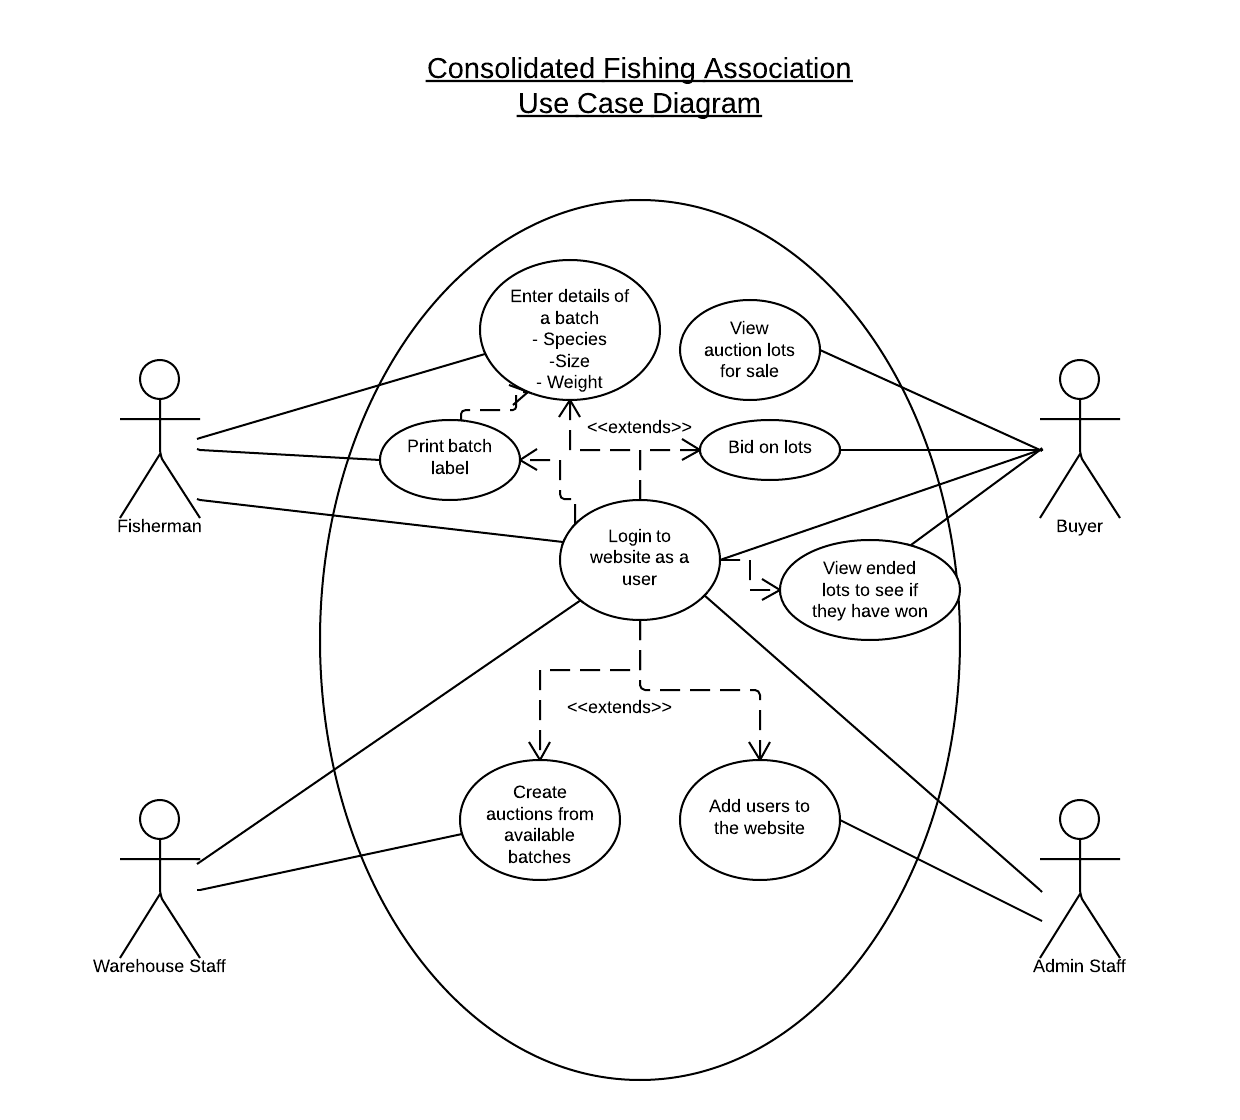
\includegraphics[width=0.8\textwidth]{img/TA-UCD1.png}
	\caption{A Use Case diagram to visually represent each users need and how they are shared or separate from one another.}
\end{figure}

As seen from the figure, each user is required to log in to the system, where they are each presented with their own different options of progressing from there, based on their particular needs and expectations on the website. This leads up to helping with the design decisions of how to best make the website design later, in order to accommodate for each different type of user, and provide them with the services they need on the same platform, without giving them access to everything or nothing.

If a user was provided with more than they needed, it would confuse them. If they were to be presented with less than they expected, they could get highly frustrated. Using this Use Case diagram, I can clearly see how each user will expect the application to look for them, and cater to their needs accordingly.

\subsection{Data flow}
When dealing with a website that handles data of different types of users, I found it good to create a diagram to represent the flow of data in the application. This ignores why or how exactly the data flows this way, and focuses on the actual flow of the data. From where does it start and where does it go to, and what is in the data. 

Doing this helped me get an idea of what the finished product would look like in the underlying data structure, and also imagine each type of user interacting with the program, and how they themselves would expect the flow of data to be on the website as a whole.
\begin{figure}[H]
	\centering
	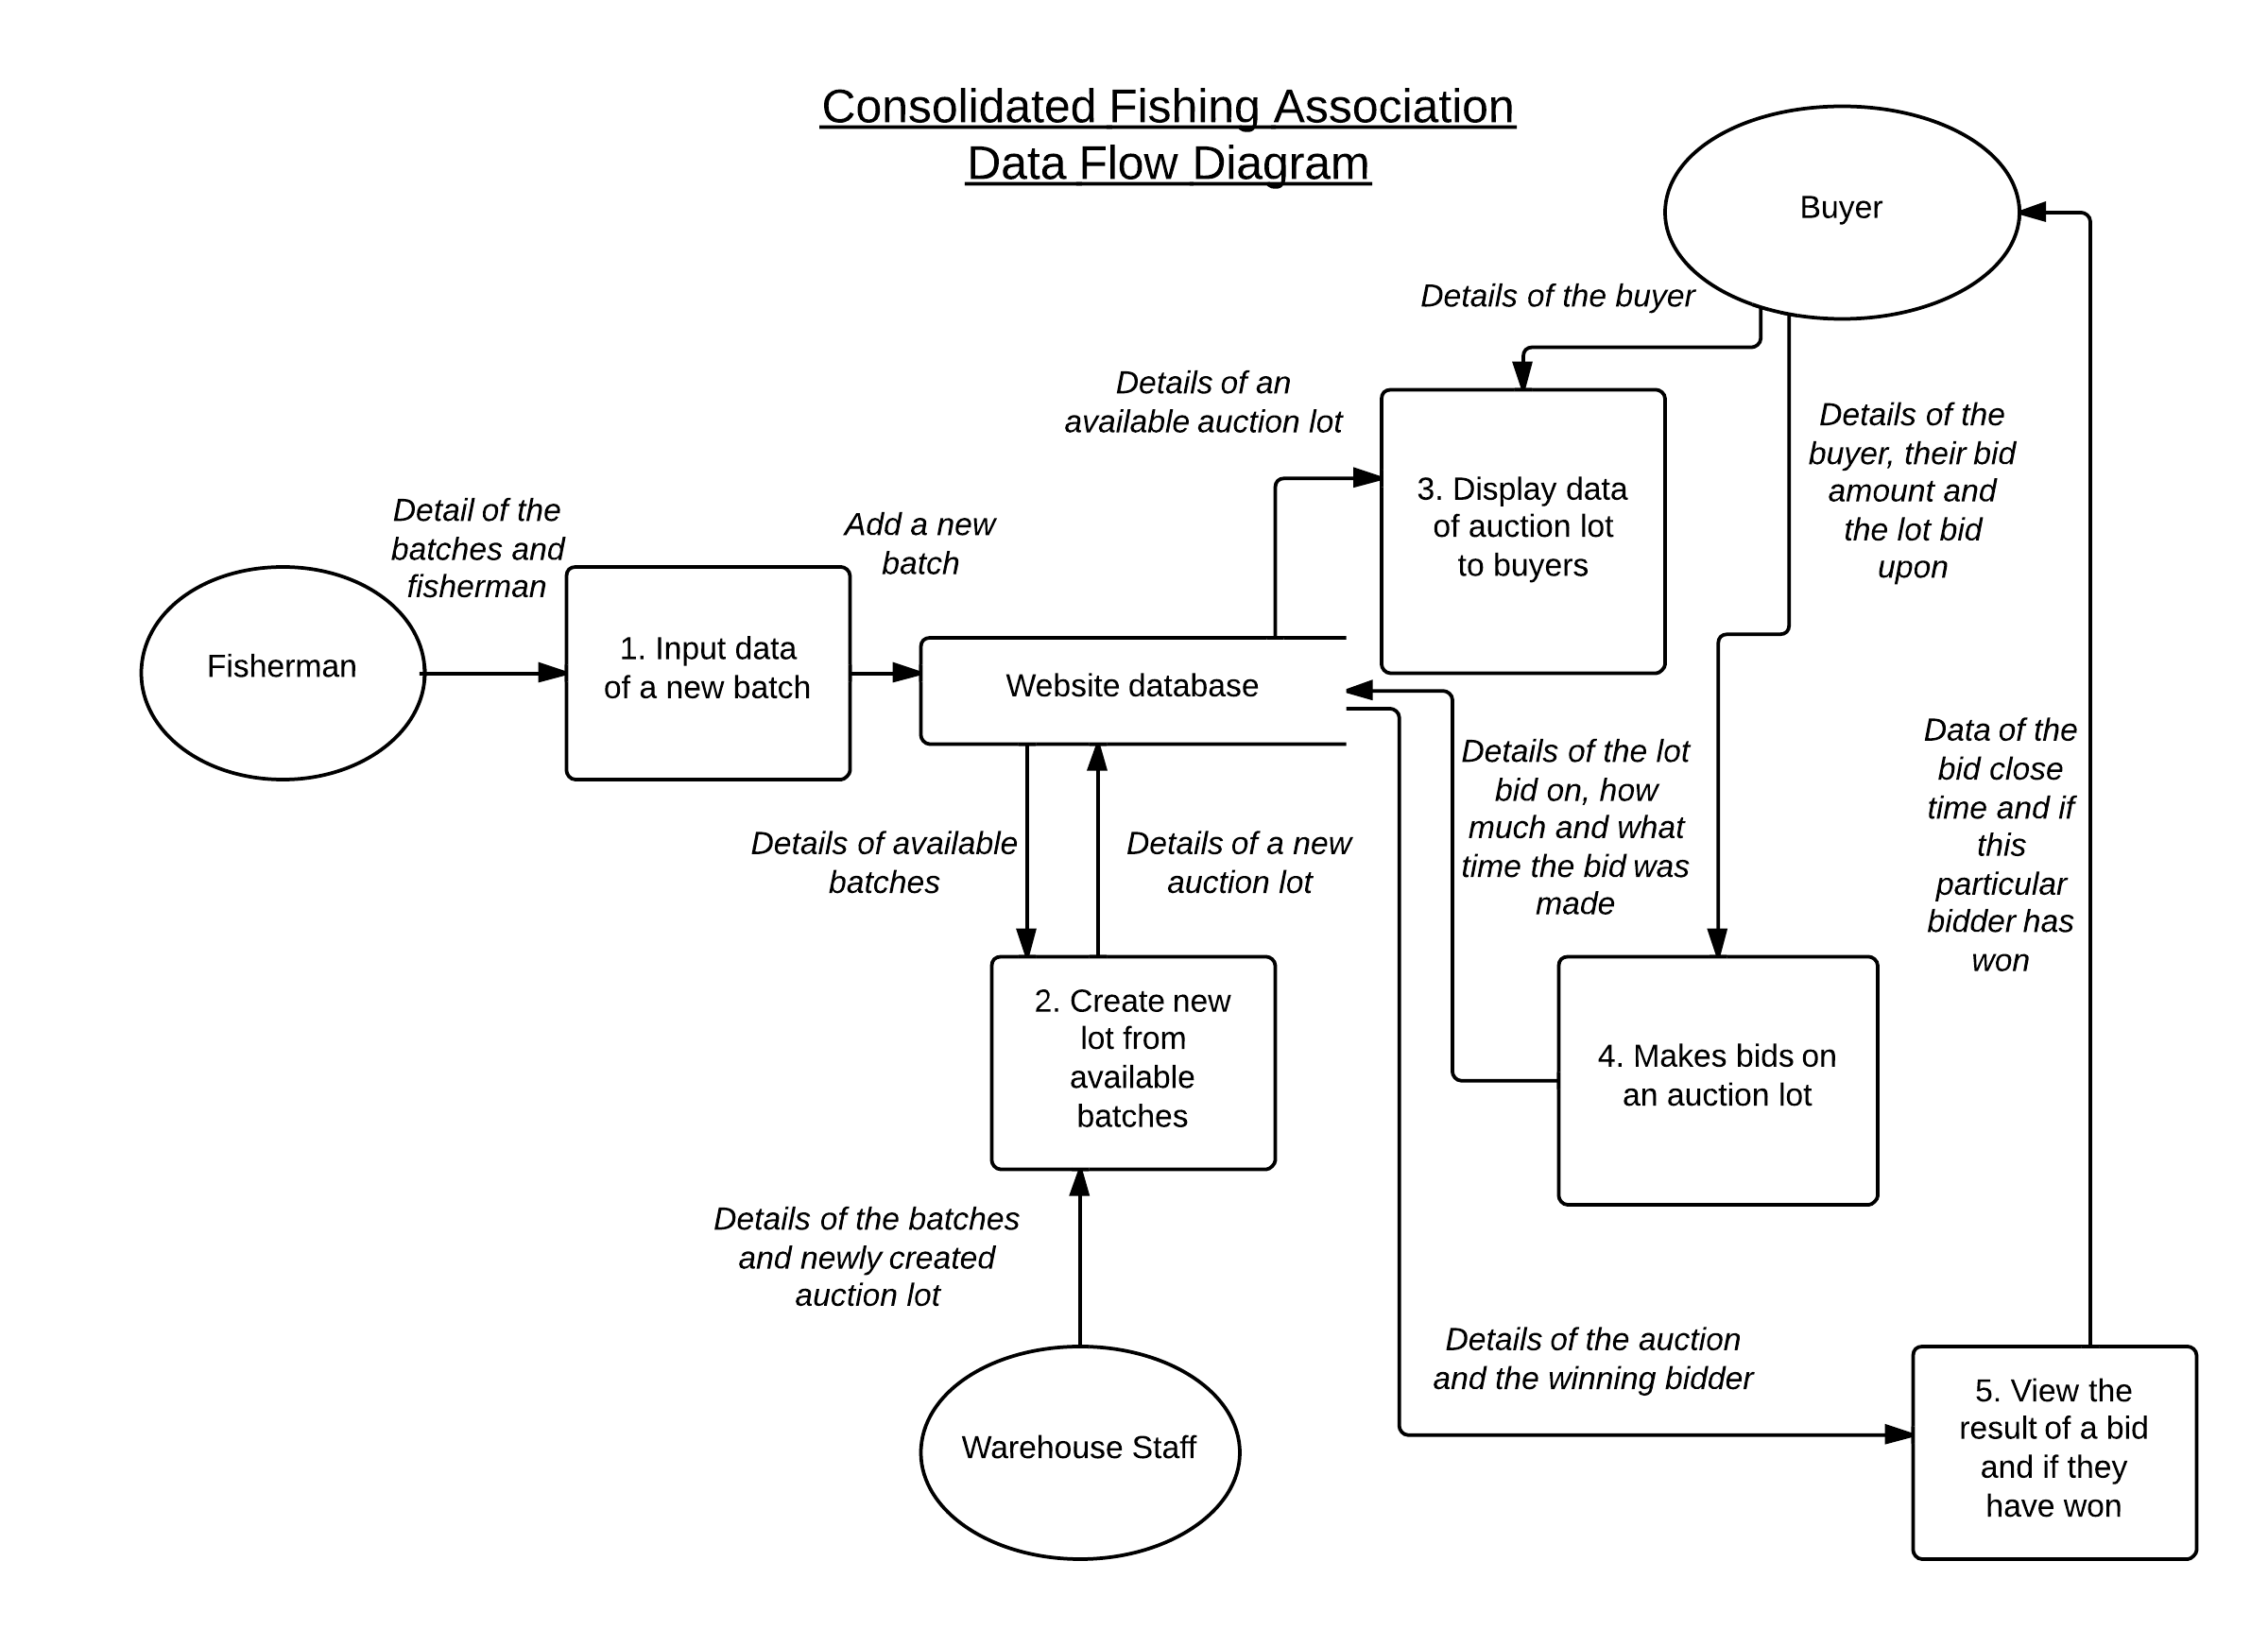
\includegraphics[width=0.8\textwidth]{img/TA-DFD-Transaction.png}
	\caption{The flow of data, as it enters the application from the Fisherman and where it travels to for each user to see.}
\end{figure}
This next figure displays the flow of data for registering a new member and the data flow in order to instate them as a member of the website with the correct access they require for their needs.
\begin{figure}[H]
	\centering
	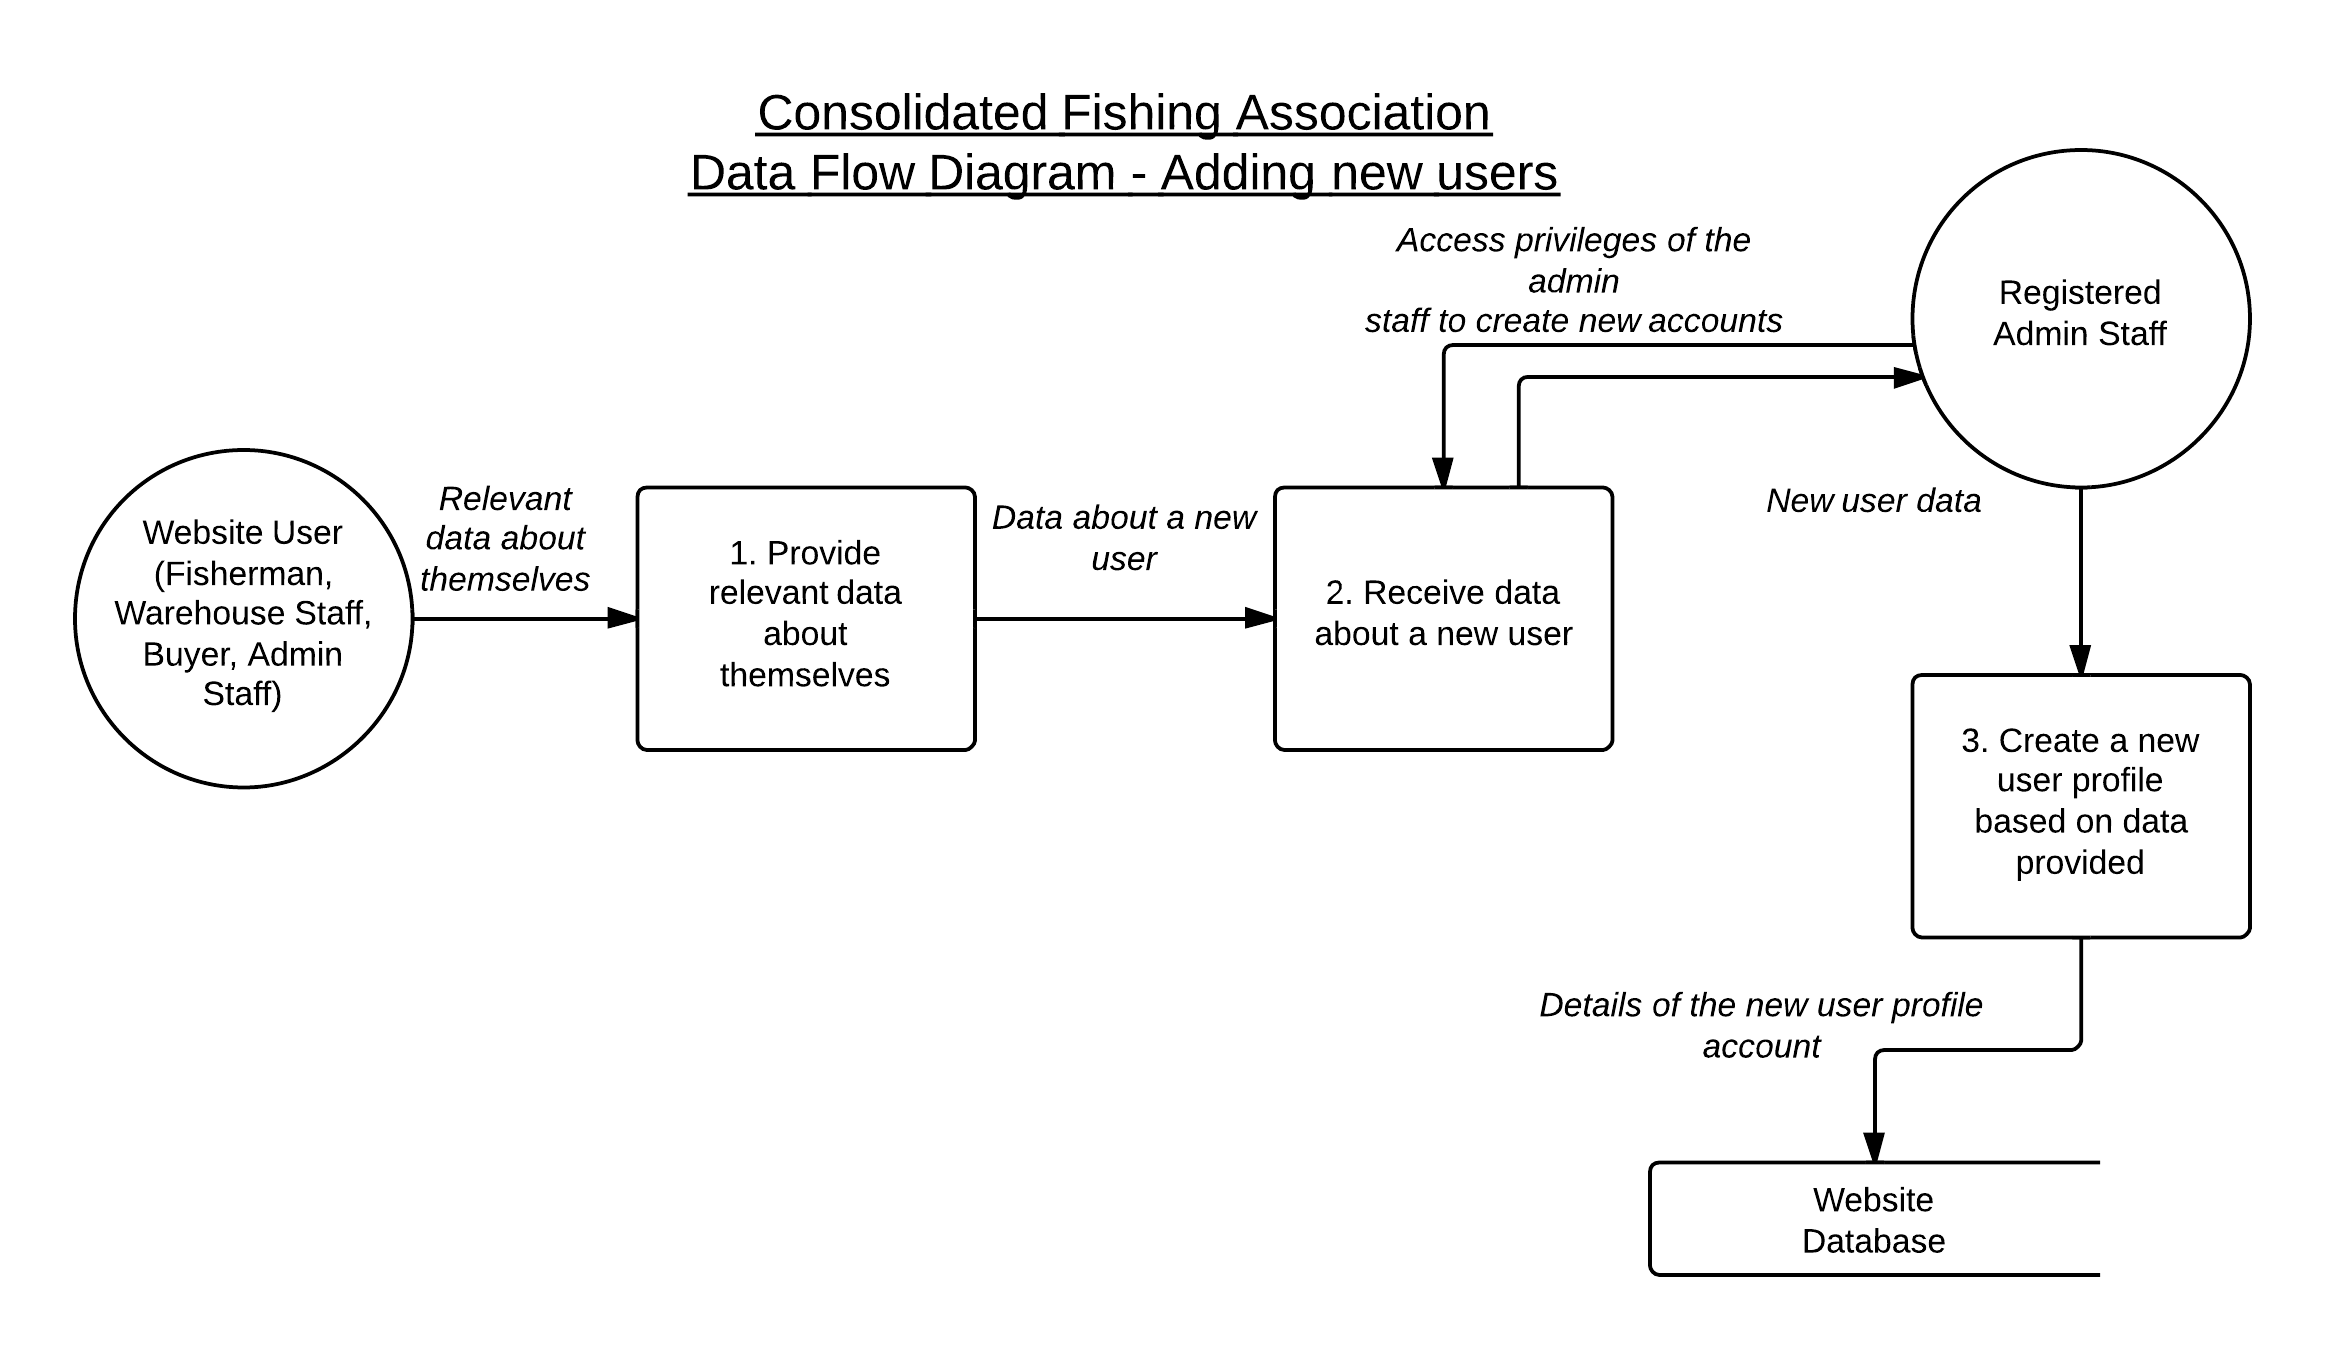
\includegraphics[width=0.7\textwidth]{img/TA-DFD-User.png}
	\caption{The flow of data, provided by the new user and passing through the application to instate them as a member on the website.}
\end{figure}

\subsection{State Transitions}
There are also a number of states that the user and the website can be in, that must be processed in order for all of the tasks that each member of the website wants to perform can be executed correctly. To demonstrate, here are some state diagrams, showing how the real world uses of the website affect the state of the website for other members of it, and how they are able to reach their needs. These diagrams also touch upon how a user of a particular type and view and use the website.

\begin{figure}[H]
	\centering
	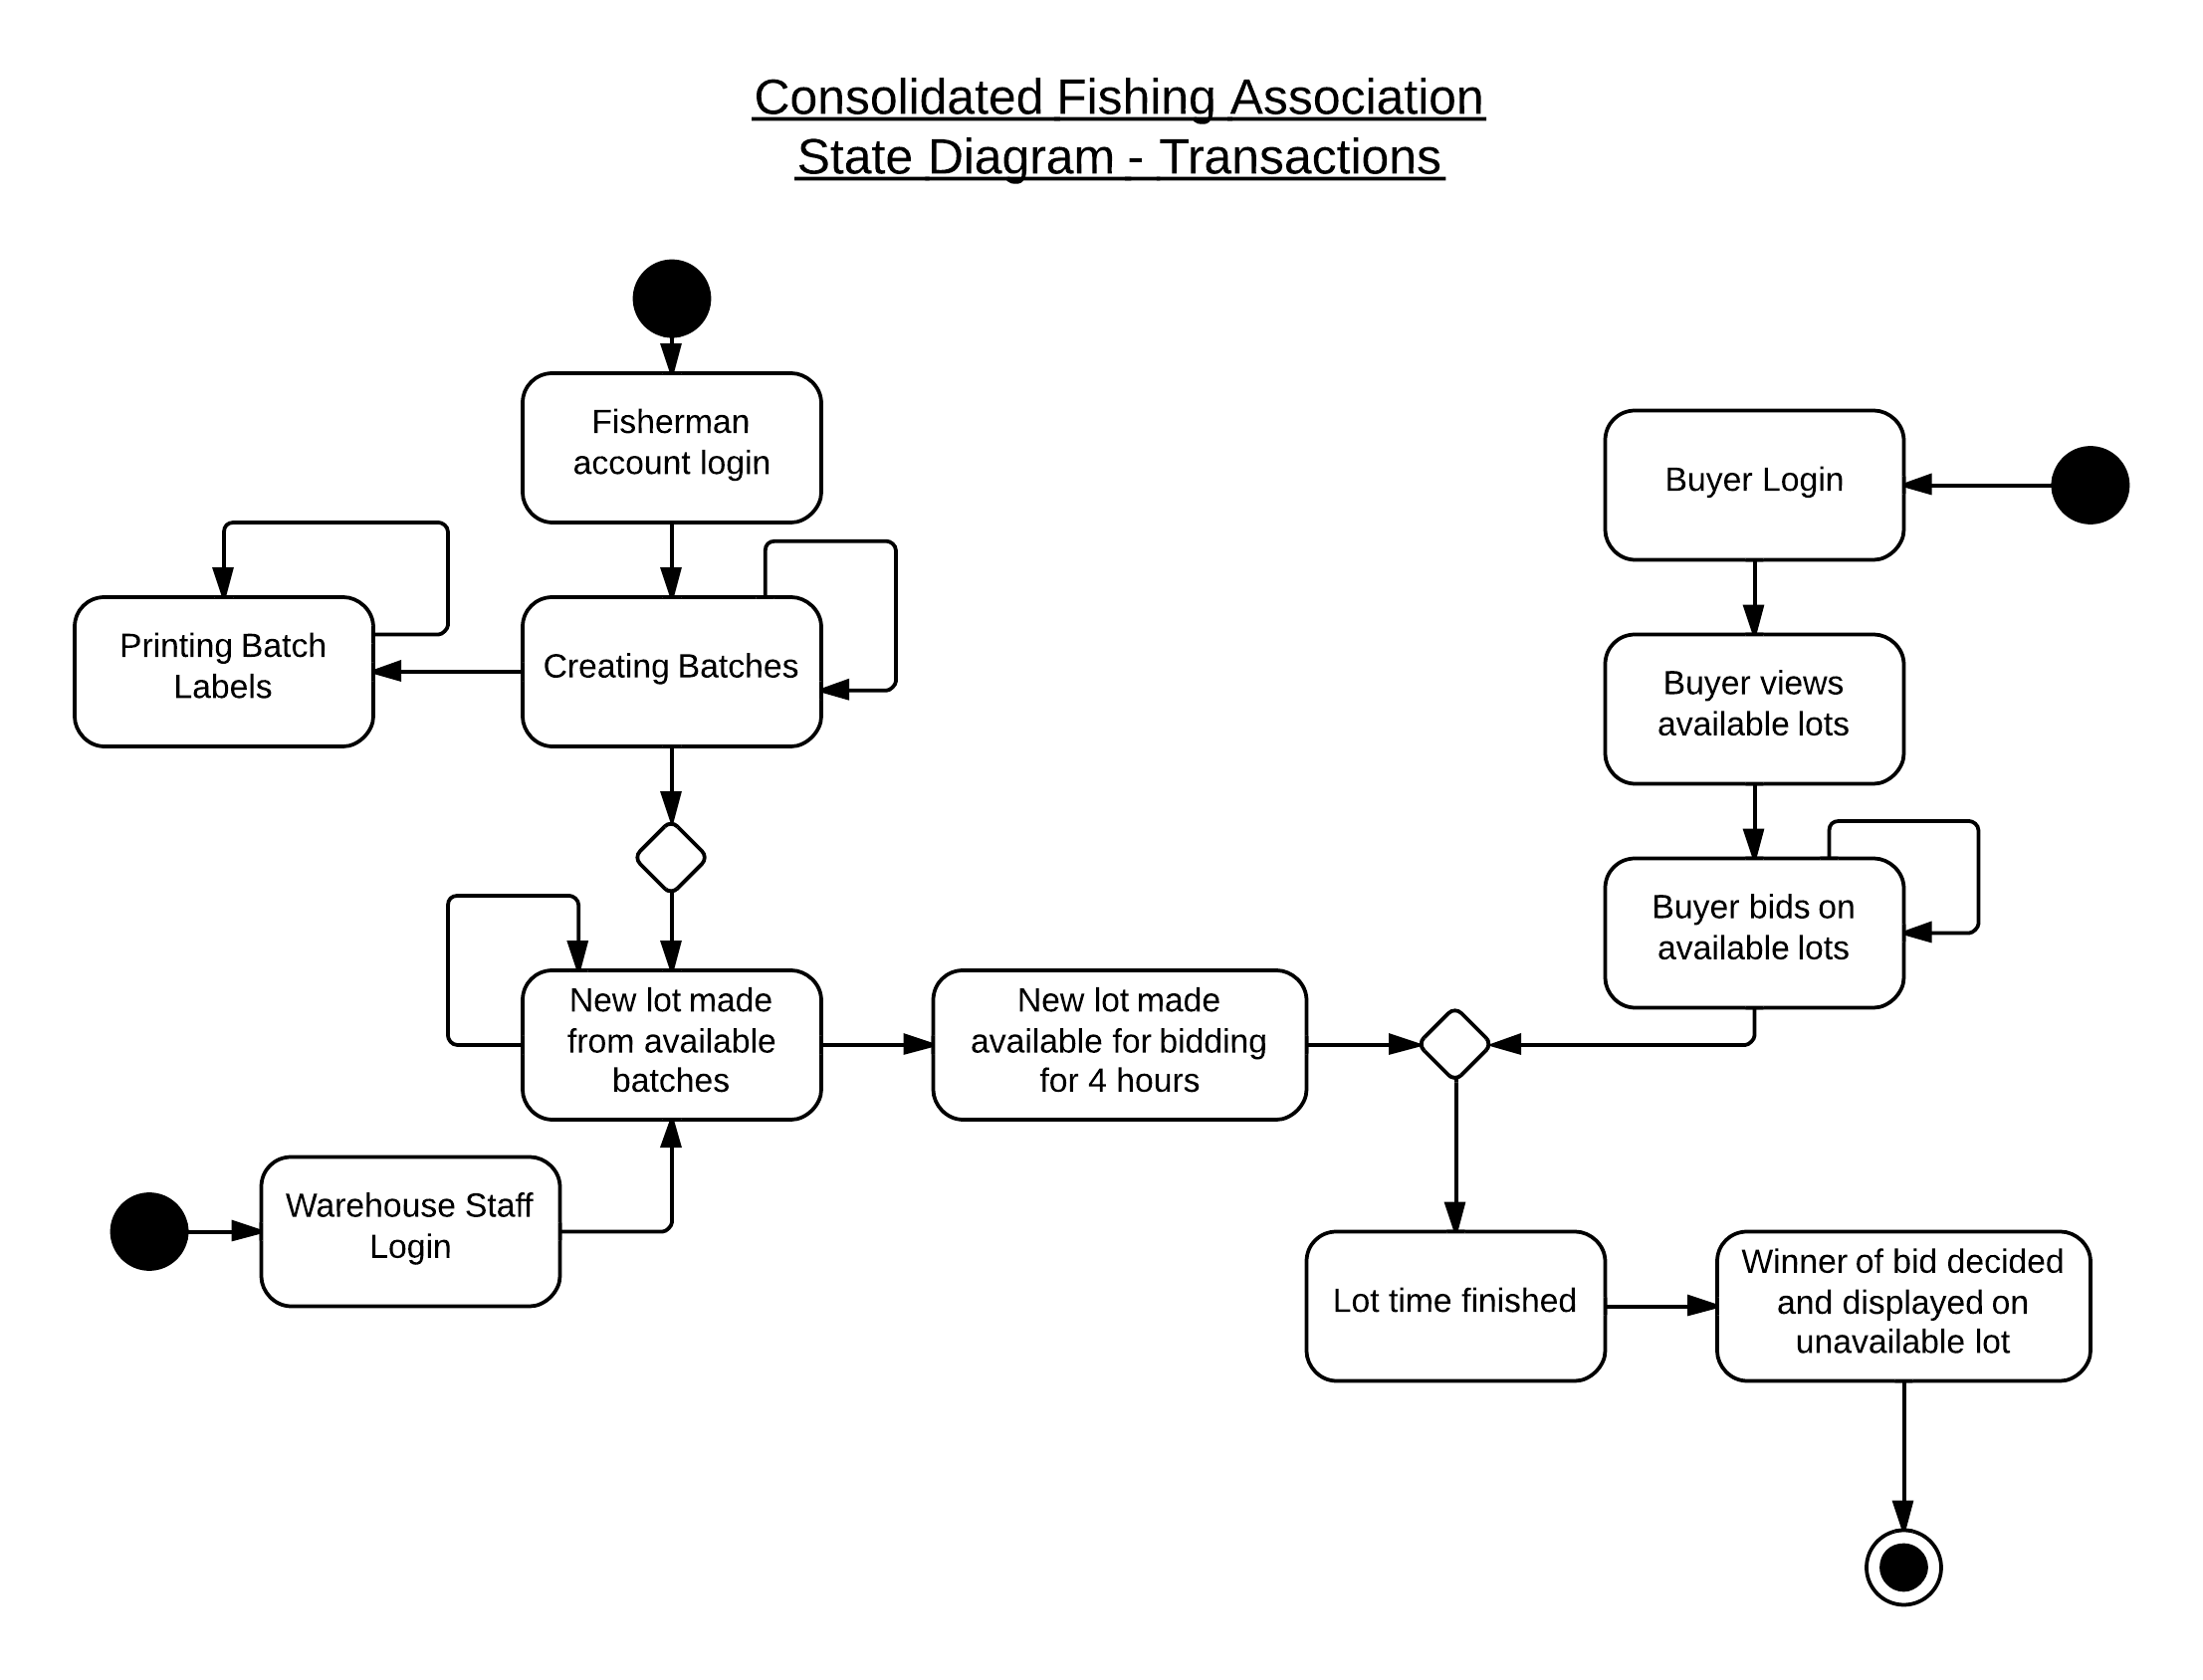
\includegraphics[width=0.7\textwidth]{img/TA-SD-Batches.png}
	\caption{The states of the process of users using the website, from the fish batches being entered into the website, to the state of fish being sold.}
\end{figure}

\begin{figure}[H]
	\centering
	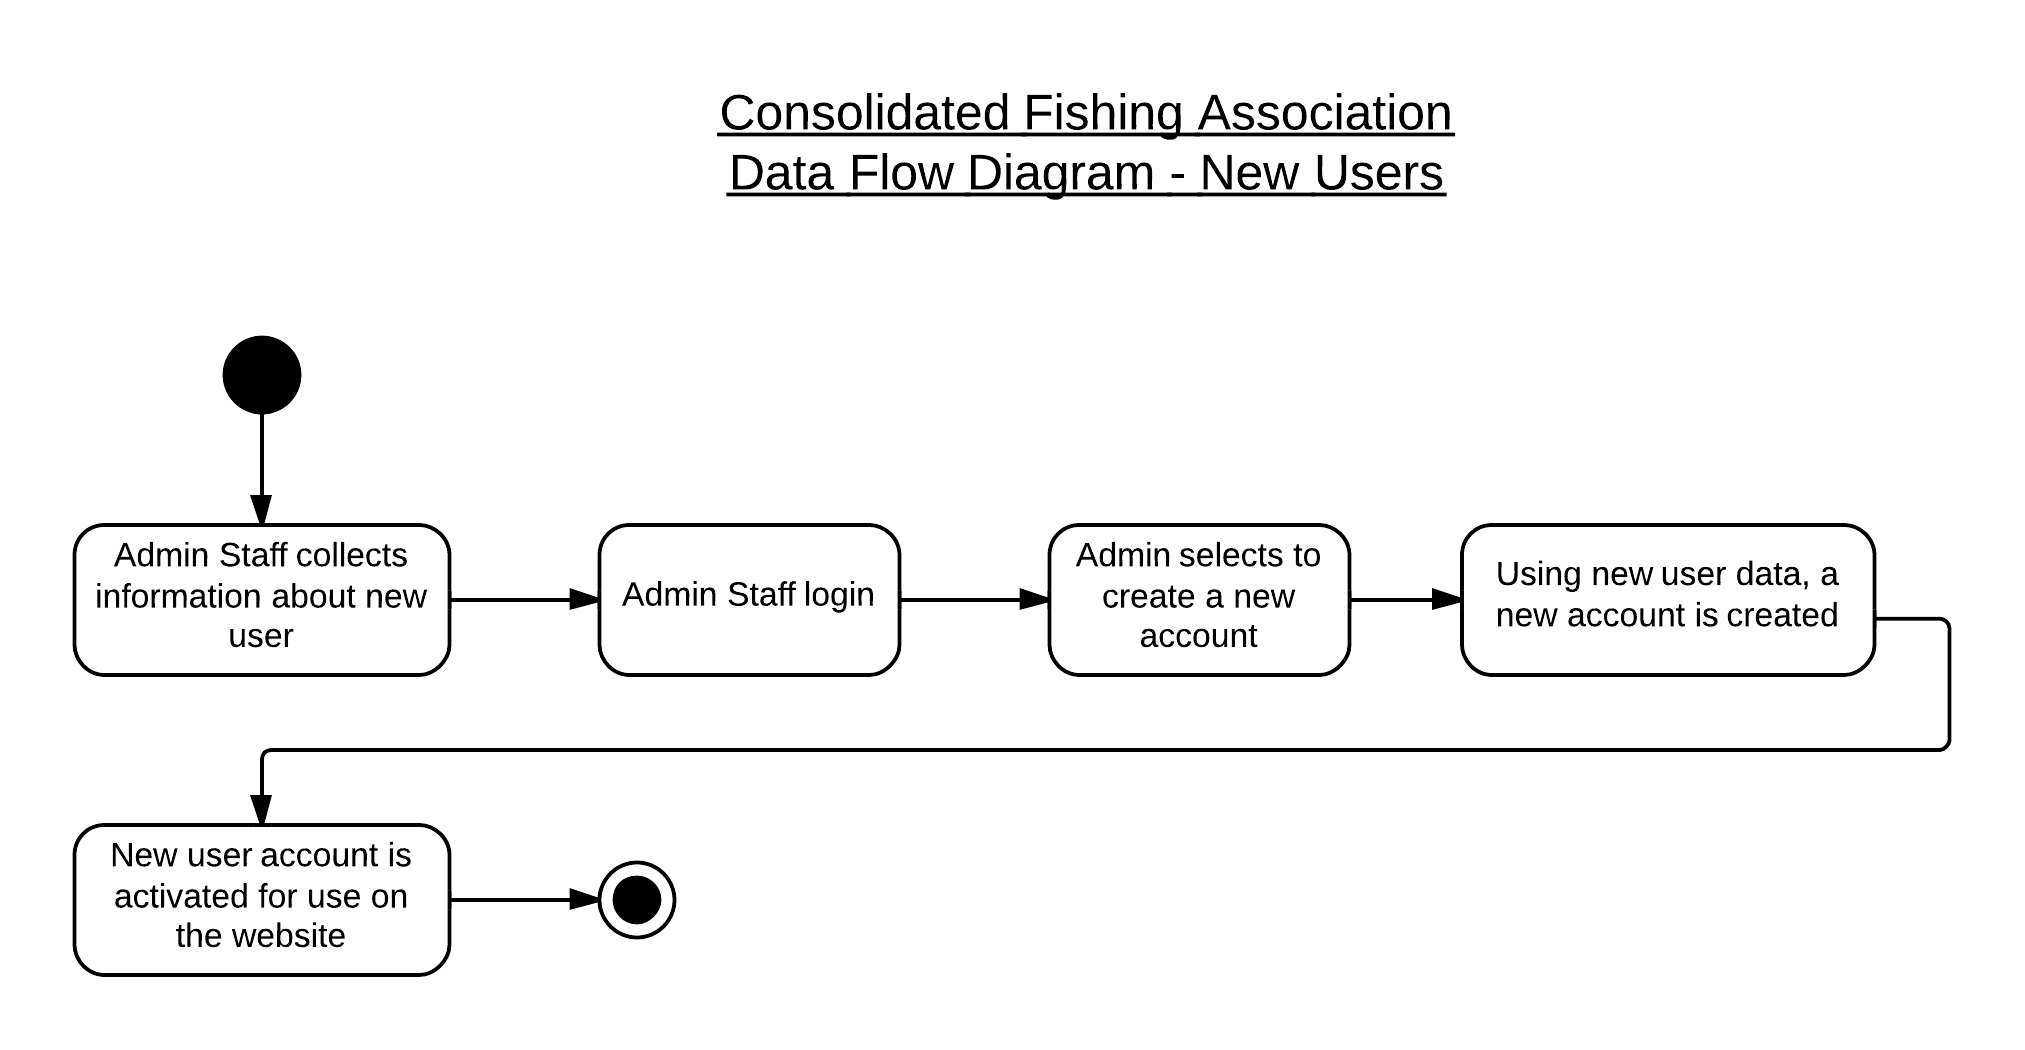
\includegraphics[width=0.7\textwidth]{img/TA-SD-Users.png}
	\caption{The states of a new account creation for the website.}
\end{figure}

Through the analysis of the tasks a user wishes to perform with the website, as set out by the requirements specification, I had a clear idea of exactly what and how the application should function. The next stage was to design the website in such a way that these expectations could be met, and give the users the best and simplest interaction with the website as possible. With the diagrams to refer to a later points, they give a solid understanding of how I had to balance the design of the website with it's usability for the target users.

%----------------------------------------------------------------------------------------
%	DESIGN
%----------------------------------------------------------------------------------------

\section{Design}
When considering the design, I had to think about the people who would be using the website and what sort of circumstances they would be under. So, for example, each user would want to find the login box relatively easily, and be able to input their username and password. For this, I planned on having a form of two boxes in the centre of the home page. Easy to access, easy to find.

For all types of account, there will be a navigation bar at the top of the screen, giving the users quick access to the home page, the ability to logout at any time and any specific requirements they have.

\begin{figure}[H]
	\centering
	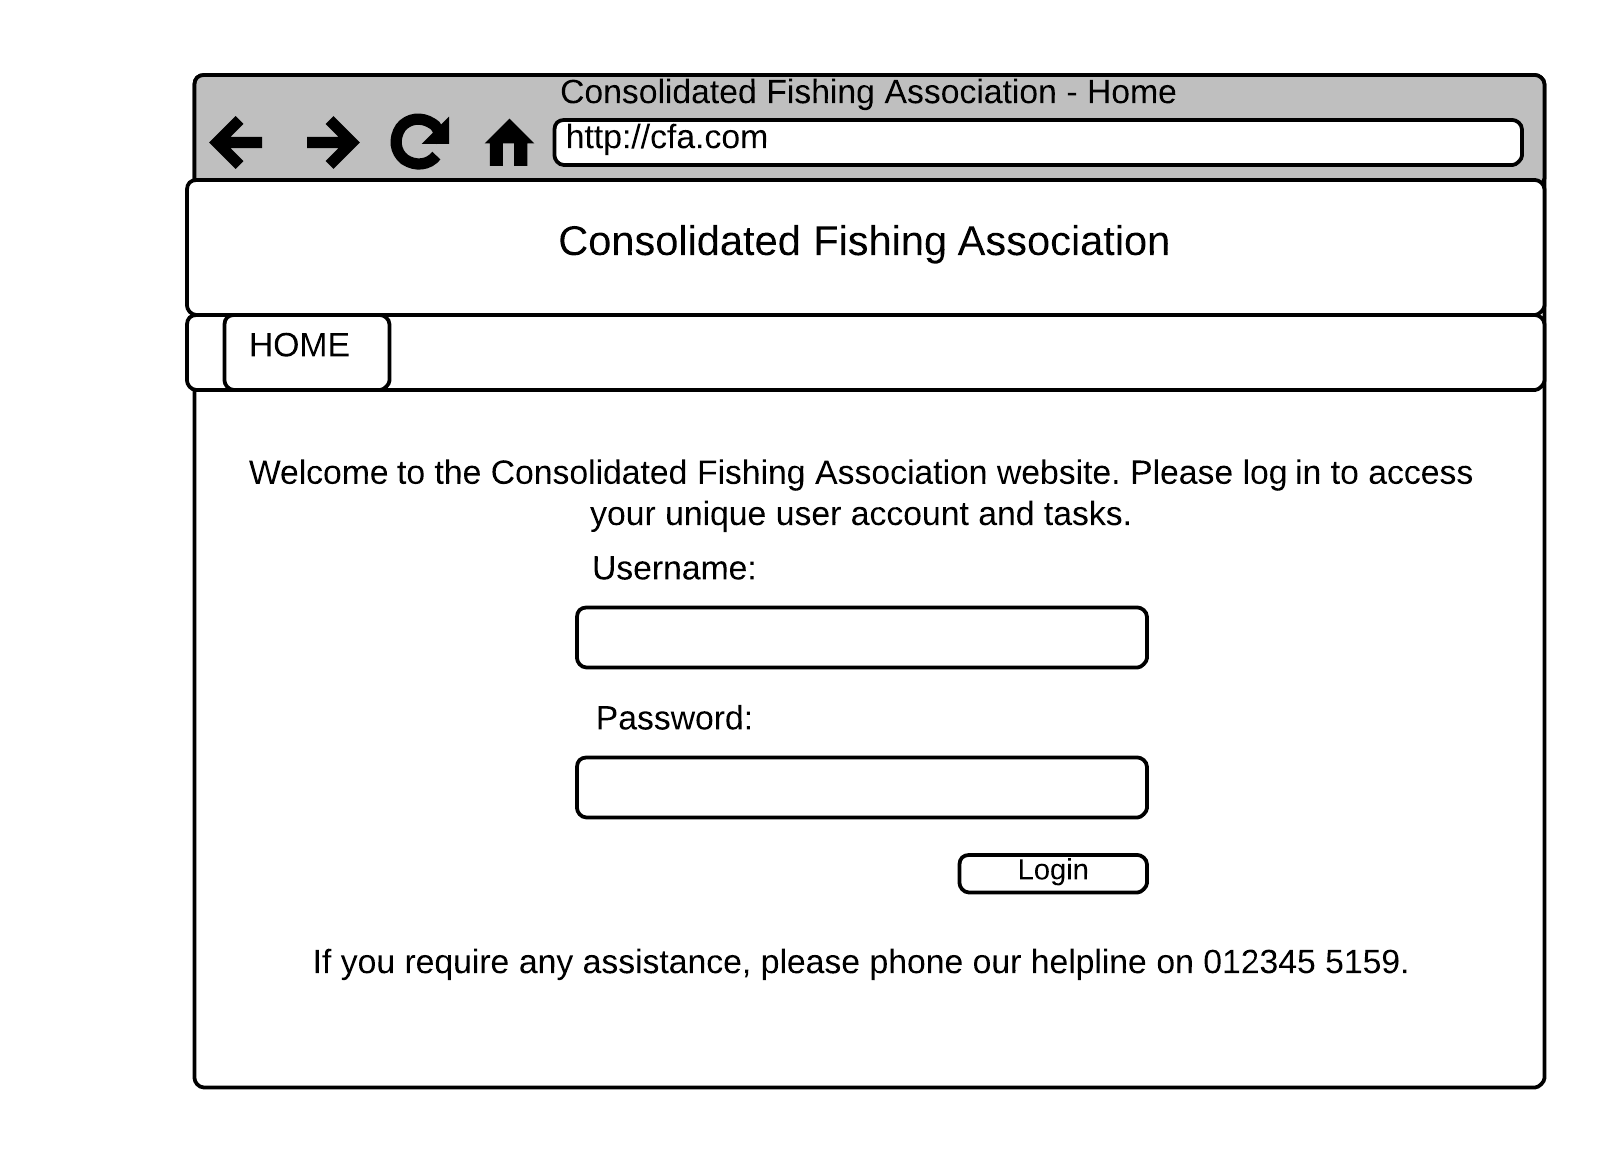
\includegraphics[width=0.7\textwidth]{img/wf1.png}
	\caption{The basic wireframe design of the Home page that all users are presented with when accessing the site for the first time from the home page.}
\end{figure}

\subsection{Fishermen}

For a Fisherman, they would want to go straight to inputting their batch information, and be able to input it with ease. For this, I chose to use drop down boxes for the different types of size and species they could select, and number entry boxes for the weight of the batches and number of crates in the batches.

\begin{figure}[H]
	\centering
	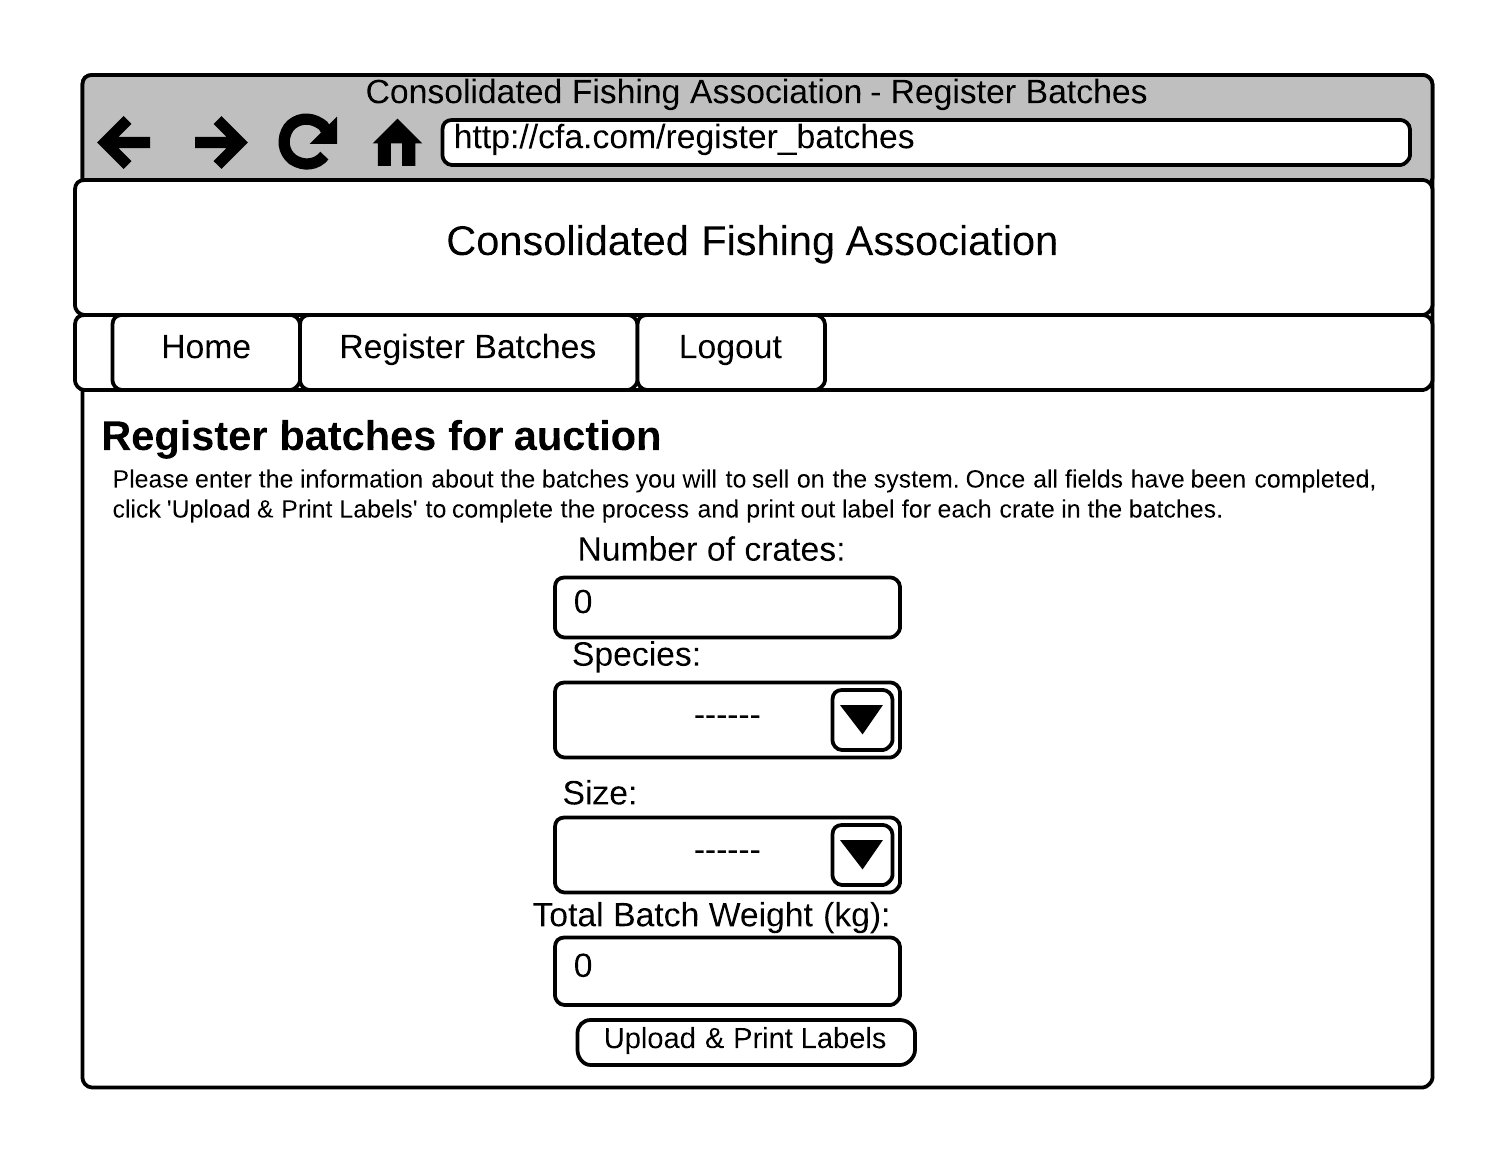
\includegraphics[width=0.7\textwidth]{img/wf2.png}
	\caption{The basic wireframe design of the page fishermen use to input their catch data. The input boxes are larger than they normally could be for ease, in the chance they may use a touch screen}
\end{figure}

Considering that the Fishermen will probably have a number of batches to get through, and may be wearing gloves and using a touchscreen to enter the data, I intended on making all boxes large enough to click on, and buttons easily recognizable, such as those buttons for printing labels. This way it makes it much easier for them to navigate through their section of the website while working, and helps them more than hinders them.

\subsection{Warehouse Staff}

A warehouse member would be using the website for combining batches into lots, so their most vital data comes from the available batches list. For this, my plan was to have an area on their user account that lists all currently available batches, where they could use drop down menus to choose to see a list of a particular species and of the same sizes.

\begin{figure}[H]
	\centering
	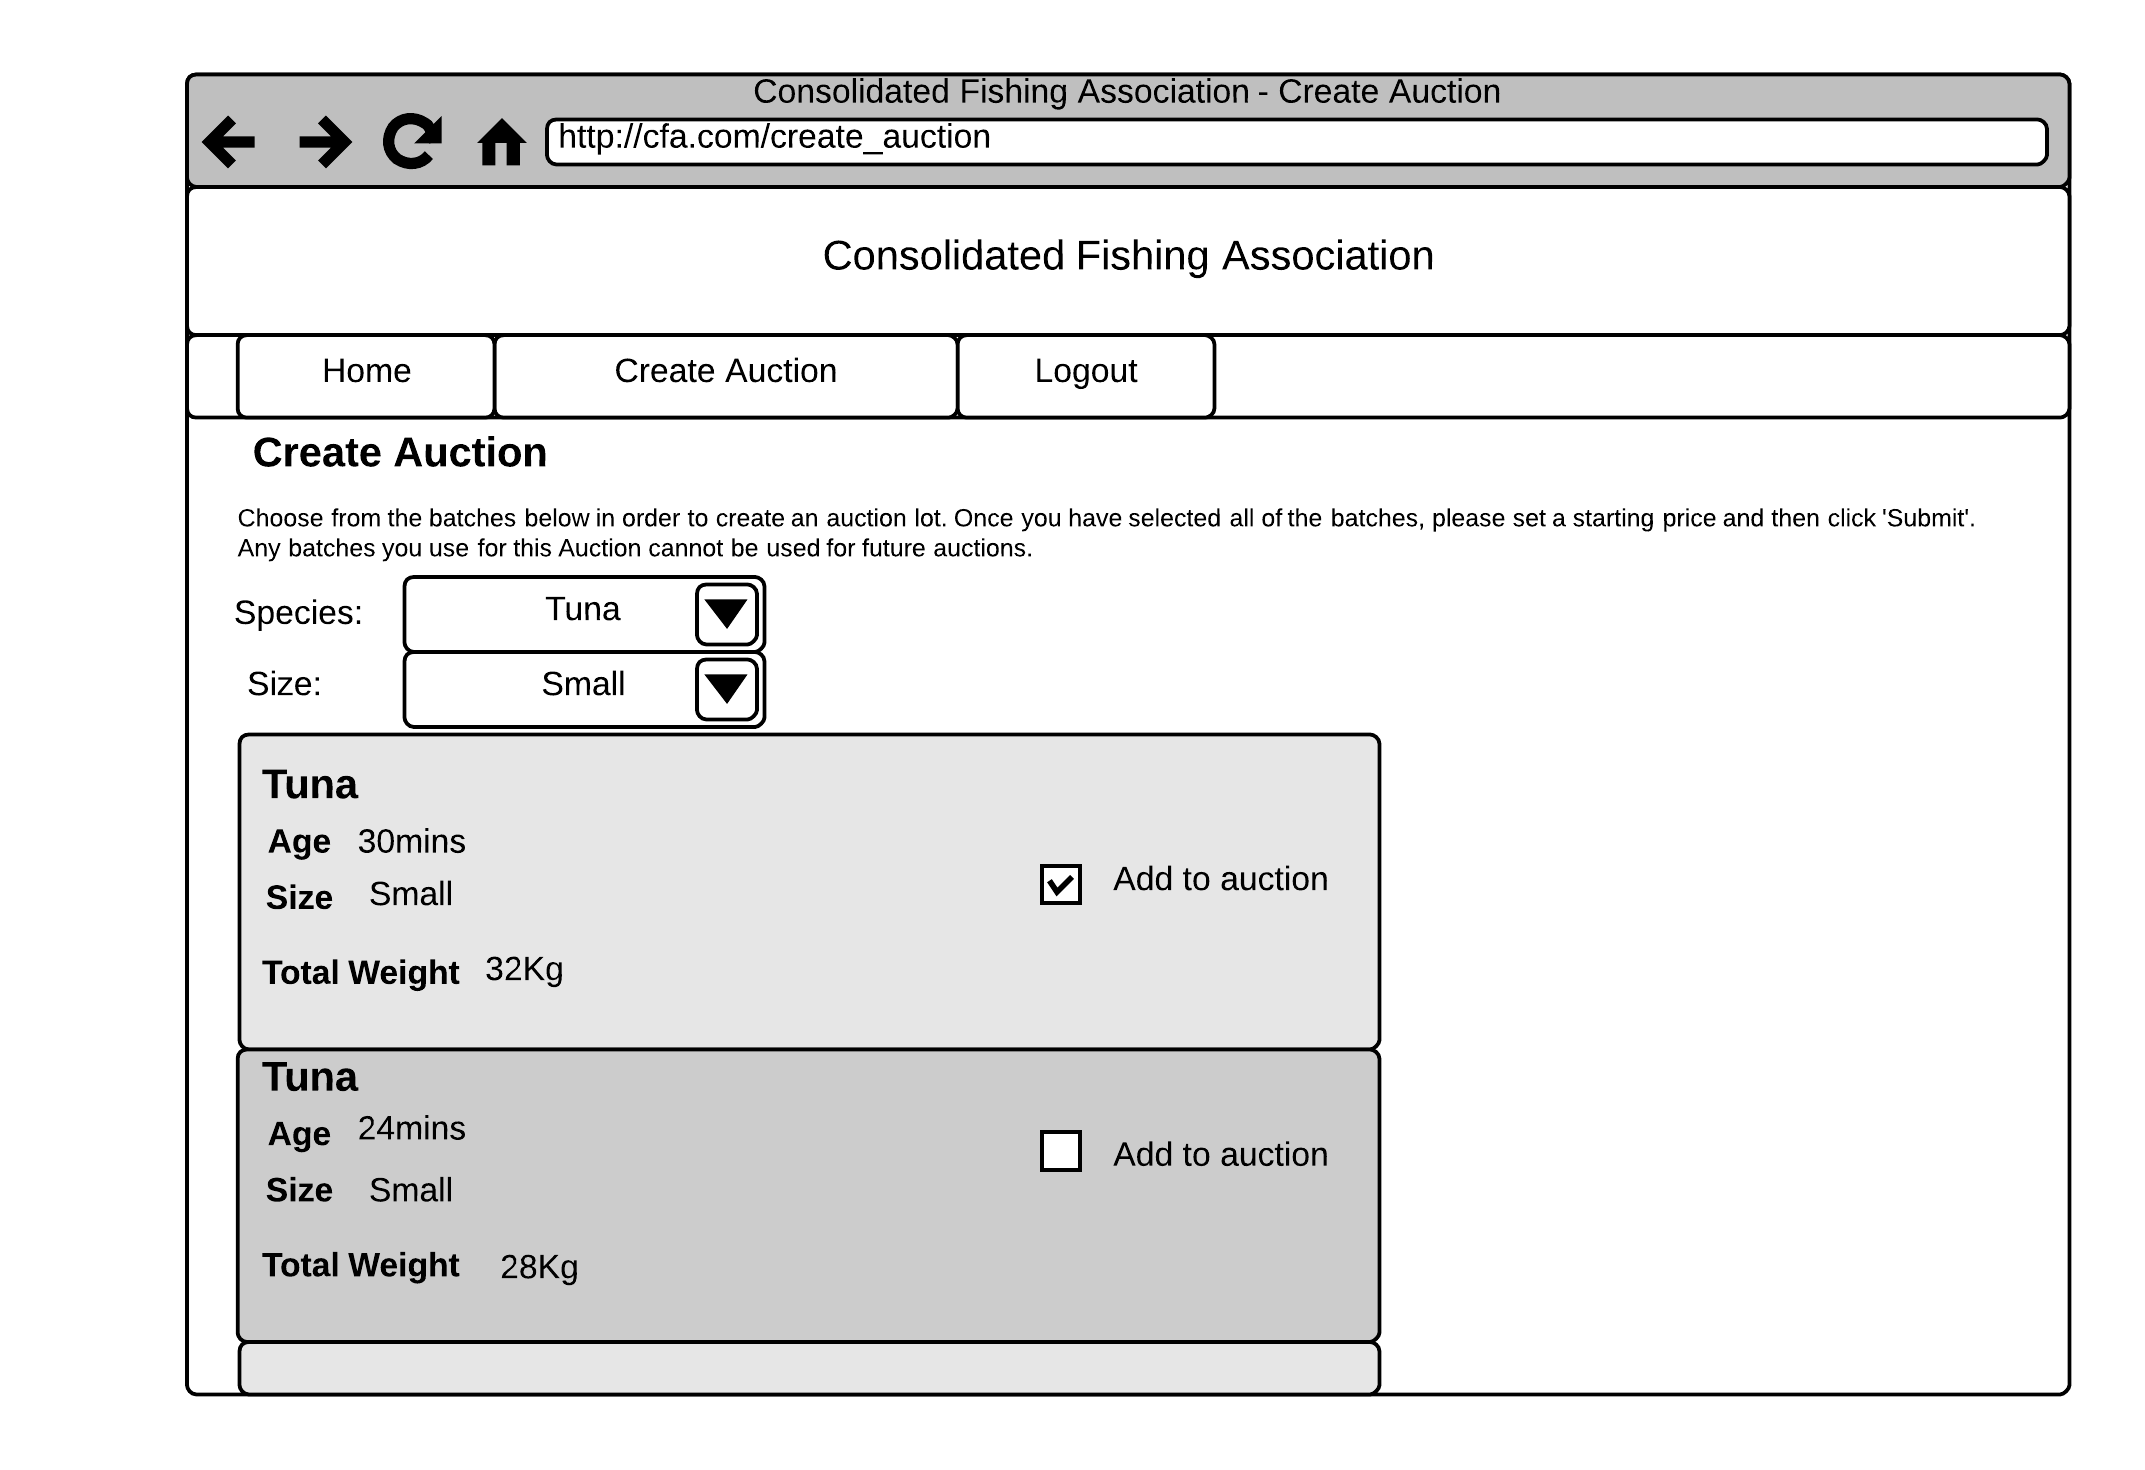
\includegraphics[width=0.7\textwidth]{img/wf3.png}
	\caption{The basic wireframe design of the page used by warehouse staff members to create new auction lots from the available batches.}
\end{figure}

In these selected lists, the fish would be listed in order of when they came in, with those that came in first at the top of the list, in order to be found and auctioned off as quickly as possible. The warehouse staff can then use check boxes next to the batches they wish to put together, set a starting price, and click to submit a new auction lot for sale to begin the 4 hour auction.

It was important in my design that the information for these section was easy to find and clearly stated, making it so that the warehouse worker does not have to work hard in order to make the system work for them. To help them with looking through a list I also decided that every second item on a list would be a slightly different colour to the others. While this may not be particular obviously helpful to the functional requirements, when you think that a warehouse user will likely be staring at the screen for half of their day, this colour change breaks up the monotony and may increase their productivity and ease of use of the software.

\subsection{Buyer}

As a buyer, their main aim on the website is to navigate to the auctions and place bids. For a buyer, their section of the website will display the current latest auctions that they may bid on, with all the relevant information, how long is left on the auction and the current highest bid. They will also be able to see a section of 'previous auctions' that they have bid upon within the past day, where they can see if they won that auction or not.

\begin{figure}[H]
	\centering
	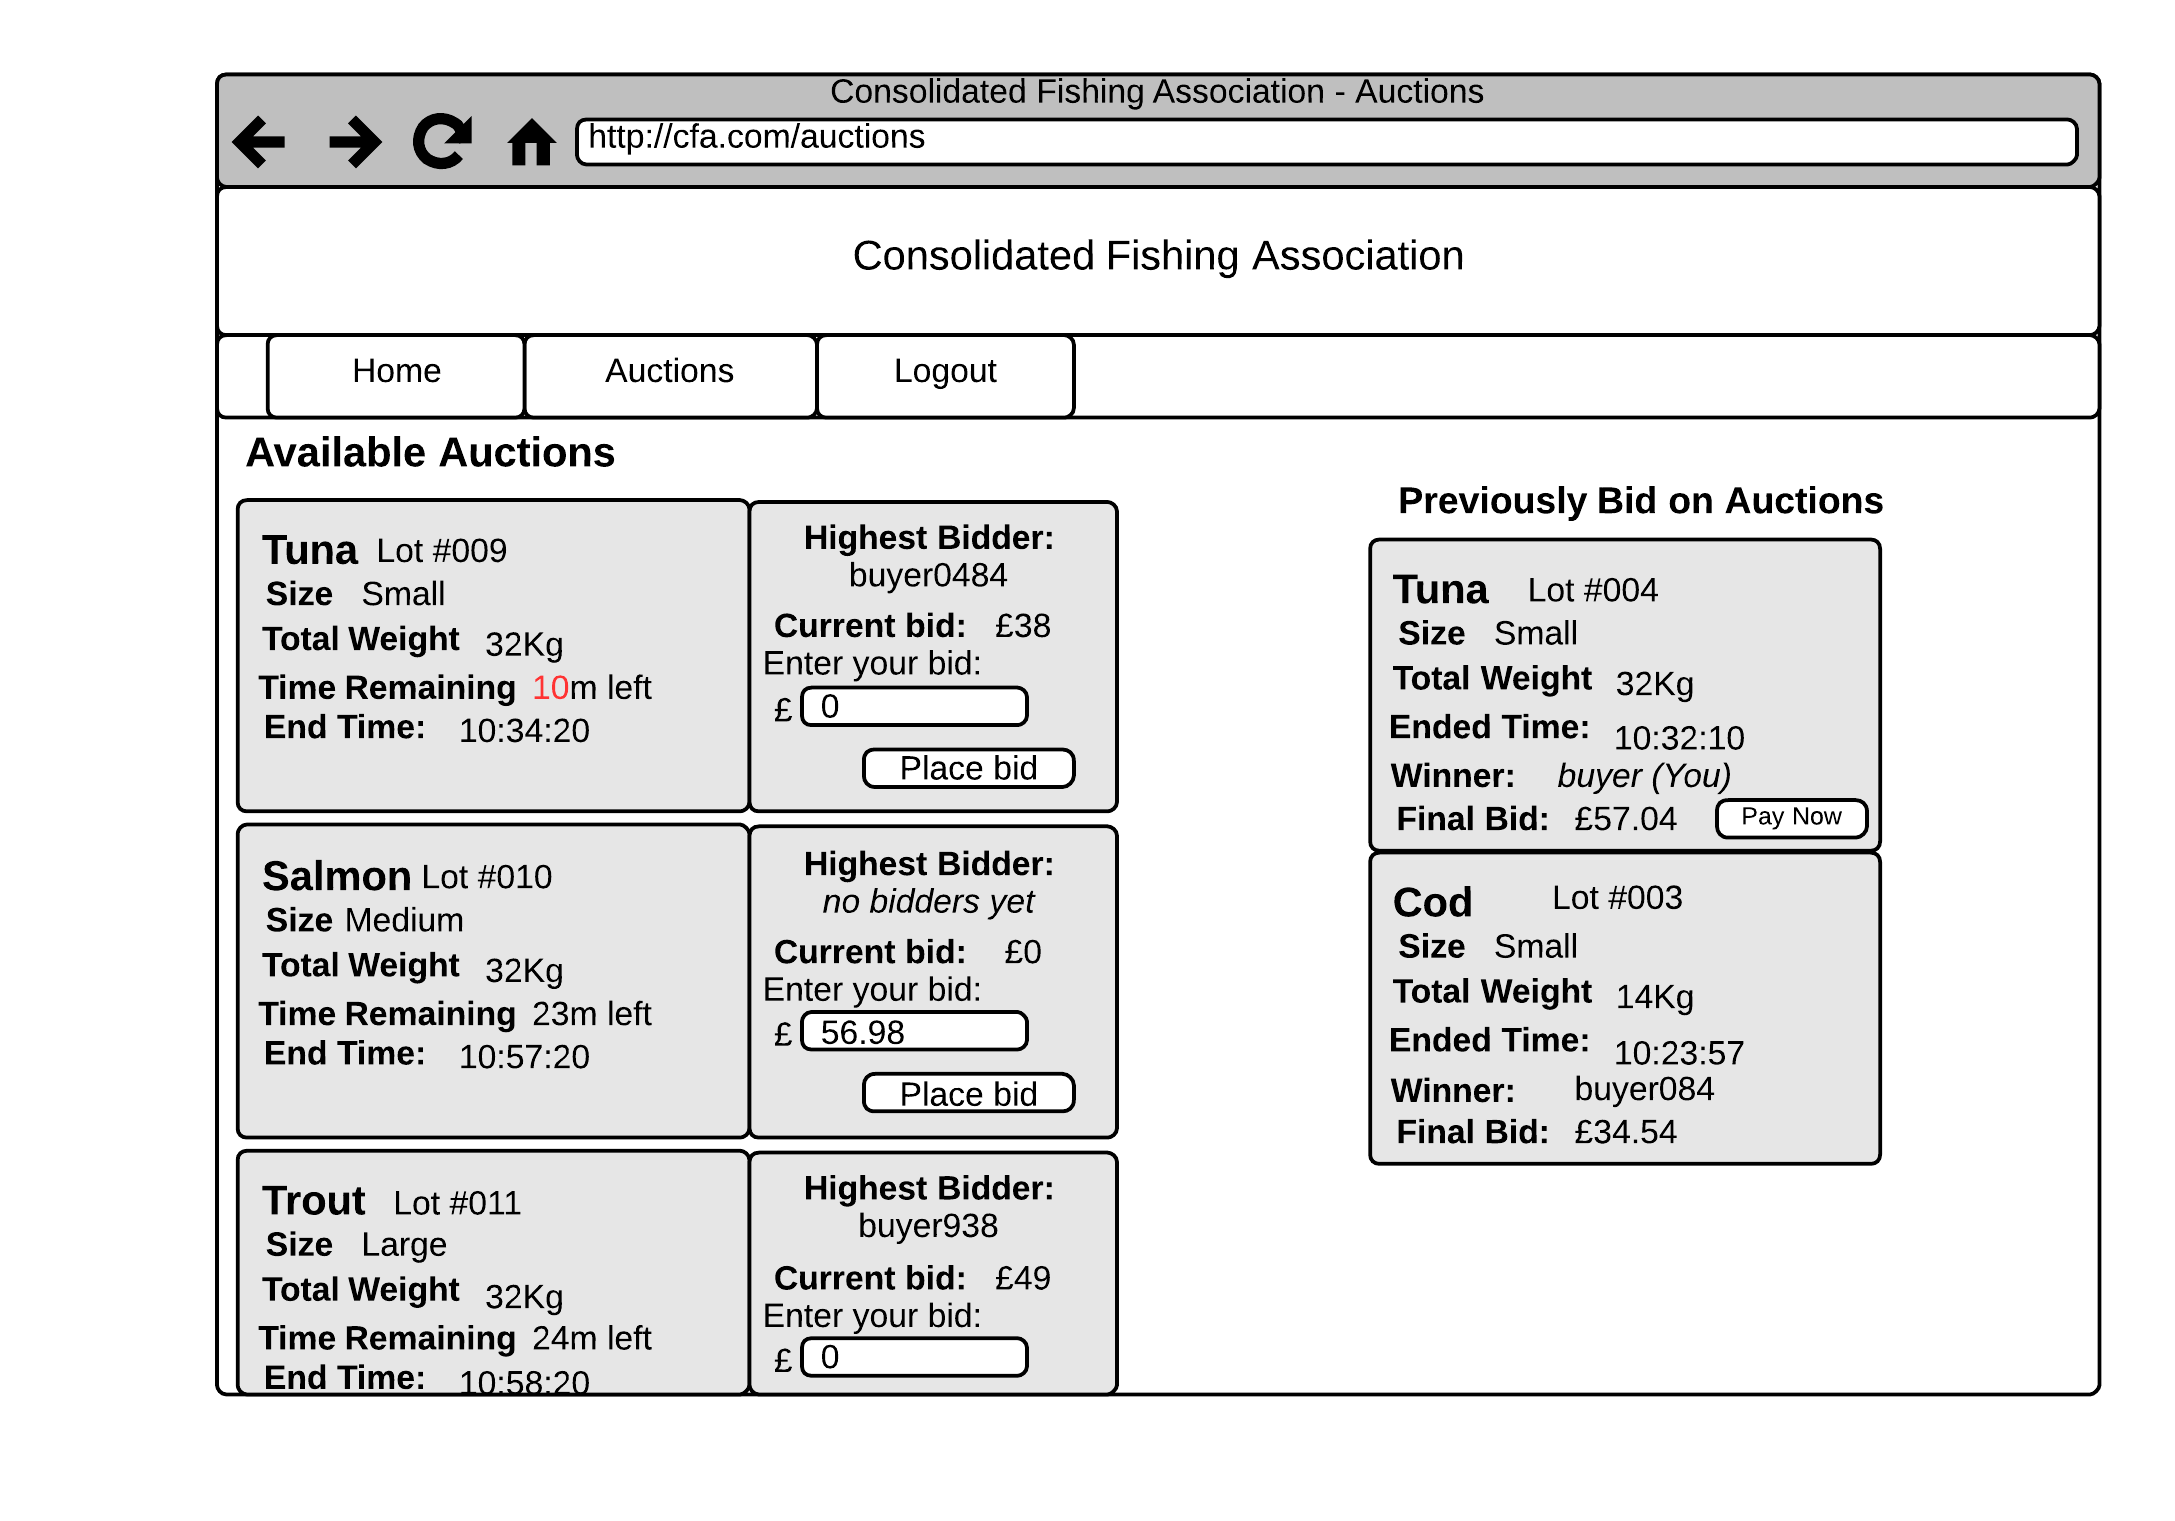
\includegraphics[width=0.7\textwidth]{img/wf4.png}
	\caption{The basic wireframe design of the Auctions screen, where a buyer may see the currently available auctions to bid on, and the results of any they have previously taken part in.}
\end{figure}

It is important for a buyer to be able to see this information, and so it is the main part of their user account: Current Auctions, Previous Auctions. To do this, their main user account will have large buttons to go to either of these sections, and each section will be a list, descending in the order of time, starting from the most recent. In order to place a bid, the user may enter a bid amount directly from the list screen.

\subsection{Administration}

Within the functional requirements, the only details provided about what an Administration staff member does is that they add new users. Since this is all I have been given, once an administrator logs in, they will instantly be presented with a screen to add a new users. They will be able to choose from a drop down menu what type of user the new user is, and be provided with a number of forms for different details, such as the user name and password. On filling out these forms, they will be able to click a Submit button and sent to a screen confirming whether the new user was created or not.

It is possible that in the future, administration staff members may want other controls, such as removing users, editing auction lots, etc. However, since this is not within the Requirements Specification, I will not be catering to it within my prototype.

%----------------------------------------------------------------------------------------
%	PROTOTYPE - Link + Brief info
%----------------------------------------------------------------------------------------

\section{Prototype}

The prototype website, based upon the results of my task analysis and the design decisions can be found at: 
\url{http://users.aber.ac.uk/jee22/cs22310/index.html}

To access the various parts of the website, you must 'login' as a user, where each user account has attached to it specific pages for handling their tasks. For the prototype, these accounts are:

Username: admin
Password: pass

Username: fishermen
Password: pass

Username: warehouse
Password: pass

Username: buyer
Password: pass

A viewer can move around the site as if it were completed, without the full implementation of the system. The majority of the forms that are on the site can be tested, although not everything will work (i.e. You cannot 'pay' for an auction, or pull up all of the different species/sizes of batches from a database when creating an auction as a 'buyer').

%----------------------------------------------------------------------------------------
%	Shneiderman's 8 GOLDERN RULES
%----------------------------------------------------------------------------------------

\section{Shneiderman’s 8 Golden Rules}
To see if my prototype was of reasonable design for a user to use with little frustration, I evaluated it against Shneiderman's 8 Golden Rules of user interface design. Through doing this, I was able to improve my prototype more, which in effect could potentially lead to a better resulting website if this were taken through to the final product release stage.

\subsection{Consistency}
The prototype is consistent in it's design and layout of the ways that a user can use the functions of the website, through doing this, a user who may have an account for both a buyer and an administrator, knows that they can access their main controls from the navigation bar in the header, and that the logout button will always be on the navigation bar at the end.

On each screen, the header always tells the user who they are logged in as, and so keeps the consistency of what account a user might be on if they are using a computer which might be shared by multiple account holders. In the prototype, this shows 'buyer', 'admin', 'fishermen' and 'warehouse'. In the release, this would show the users actual account name.

\subsection{Shortcuts}
The sections that each individual user has access to are all relatively easy to access, and can be reached in one or two pages maximum. As the website it expands, it may be worthwhile including a break crumb trail, or a search bar, in order to help a user quickly find the page they require. For now though, all of the information they need to complete their tasks is so easy to reach that they are not required.

Also in release, to help frequent users, it would be worthwhile adding a 'Remember me' check box to the login, allowing a user to leave the website entirely, and return at a later stage already logged in.

\subsection{Informative Feedback}
On each action a user can take in the prototype, there is often some form of feedback that they have completed a task. Examples of this are such as placing a bid on an auction item as a buyer. When they click to place a bid, they are first asked if the amount they want to bid is correct. If they confirm, a number of things can happen. If the amount they enter is too low, they will be told so. However if it is correct, they user will instantly see their bid has been placed and that they are now the new highest bidder.

\subsection{Closure Dialog}
There is closure in the prototype for areas where the user has followed a series of steps to do something, and then reaches a conclusion. An example of this is when an administrator user creates an account on the website, but then might realize they have made a mistake. One the screen confirming that they have made the account, there is a button to 'Undo' the account creation. By clicking this, they are prompted to ask if they are sure they want to Undo the account creation. When they hit 'Yes', the account is removed (in full release), and a message in red is displayed to the user on the page they are on saying that  the account they have just made has now been removed.

This message provides the user with the feedback  that their action has been completed, and that they were sure it was the action they wanted to do. Through this, the user gets closure that their task has successfully been completed, and the account creation reversed. On the same page there is also a button to create a new account, so they can click this and be taken to the account creation page, bringing them back safely full circle.

\subsection{Error Handling}
With a website handling currency and sensitive information, it is important that there is robust error handling. For the prototype, this comes in the forms of checking that user input is correct, or that the user hasn't tried to process something without any actual data to process.

For an administrator, this means that no fields can be blank. They must use a correctly formatted e-mail address, that follows the e-mail style conventions (@ .), and that when they enter for a new user password, they must enter it twice, to be sure that they entered the password correctly.

Fishermen are unable to create new batches without filling in all of the needed information. A warehouse memeber cannot make auction lots from batches without selecting at least one batch. A buyer cannot place a bid onto an auction lot without first entering an amount to bid that is higher than the previous bid amount. trying to do so will result in their task being stopped and they will be informed of their mistake.

\subsection{Action Reversal}
Many actions in the prototype can be reversed. The main ones are that an administrator can undo the creation of an account, in case they made a mistake with some of the information provided, and fishermen can undo the creation of batch if they also made an error in their data entry. This is easy to do, through the click of a button after the creation, and they will be asked to confirm if that is what they do want to do.

On the other hand, I have not allowed a user to undo something such as placing a bid on an item. I feel that doing this would be counter-productive to the system, and that asking the user for confirmation before bidding is enough. If a user were able to undo a bid on an item, it might confuse other bidders, who see the latest bid raise, then fall again, and so could be used to exploit the system.

\subsection{Internal Locus of Control}
The prototype makes the user feel in control, as any action they take gives them a response, and the system expects the user to control the flow of what happens while they are on the website. The only time the user is prompted for a response is when they themselves have already pushed for an action. This can be seen on occasions like when a buyer is bidding on a lot by their own choice and are then asked to confirm if this is their decision, giving them the control and power over the steps taken.

\subsection{Short-Term Memory Load Reduction}
In order to reduce memory load on the users, the information that  they need for a page is consolidated onto a single page. The best example of this is on the buyer Auctions page. Here, they may see any currently running auctions on the left, where they may bid and keep their eyes on them, while on the right hand side, a little smaller, they can see what auctions they have previously bid on. By keeping these bits of content grouped together, it allows the user to remember what they have bid on and won, while giving them the chance to bid on other items at the same time.

Since it is possible a user might be trying to fill some stock inventory, and have a mental list of what they want, having these two sections together can be a great help to them. It allows them not to have to focus on a mental checklist so much of what they have previously won or perhaps bid on and lost, and instead see them right next to where they might try and win another new lot.

A smaller but similar example, is how an administrator user enters all information about a new user account on the same page. It is possible that each part of the user information could be included on a new page. However, by group it all in one place, the admin can easily see what fields they have already filled out and which are still to be completed, reducing their short-term memory load by keeping everything they need to be aware of right in front of them.

%====================
%     REFLECTION
%====================

\section{Reflection}
The resulting prototype I have created, based upon the requirements specification provided with the assignment brief has been built on my task analysis and design decisions, formed through thinking of how a user would need to interact with the website. It has been evaluated against Shneiderman's 8 golden rules, and has been changed to ensure that it follows these rules. In regards to all this, I feel that my prototype is an acceptable prototype for the task set, and that it paves a clear way for the potential future release version of the website.

That is not to say that there are not improvements that could be made on the website, however. There are a number of features and sections of functionality that I can think of that have not been included in the prototype. An administration user might want to see a full list of all accounts and be able to delete and edit them from this list. This wasn't included in the requirements specification though, and so it also wasn't included in the prototype. I feel this is something that could further improve the usability of the website.

Similarly, if more pages were to be added, it would be worthwhile to include a 'breadcrumb' trail, displaying where the user started their navigation (HOME) on the website, to where they currently are, with links leading back through the pages they would have taken to reach the point they are at. With the website in it's current state though, I did not feel this was necessary to be included, and in a real world situation, saving time by not adding currently unnecessary features also saves money. I felt it was a fair choice to leave out aspects like this and a search bar.

With what was provided in the requirements specification, I believe my prototype website meets the expectations of the tasks that it's users would want to do on and with the website. I think that through my designs, I have planned to ease user navigation through what they need and attempted to keep any frustrations to a minimum.

%----------------------------------------------------------------------------------------
\clearpage

%----------------------------------------------------------------------------------------
%	REFERENCES
%----------------------------------------------------------------------------------------

\begin{thebibliography}{1}

\bibitem{assignment} N. Hardy, "Fishing Association Project Requirements Specification", CS22310 Assignment 2014, 17th March 2014

%\bibitem{w3c} W3schools.com (Accessed 18/04/2014) JavaScript Tutorial [Online]. Available: http://www.w3schools.com/js/



\end{thebibliography}


\end{document}


